\documentclass[aspectratio=169,11pt]{beamer}
\usepackage{beamerucad}
\usepackage{listings}
\definecolor{ckw}{HTML}{2563AB}\definecolor{cst}{HTML}{2E8B57}\definecolor{ccm}{HTML}{8A8F98}
\lstdefinestyle{py}{language=Python,basicstyle=\ttfamily\footnotesize,
 keywordstyle=\color{ckw}\bfseries,stringstyle=\color{cst},commentstyle=\color{ccm}\itshape,
 showstringspaces=false,columns=fullflexible,keepspaces=true,
 backgroundcolor=\color{ucadband!8},frame=leftline,framerule=2.5pt,rulecolor=\color{ucadband},
 xleftmargin=8pt,aboveskip=3pt,belowskip=1pt,basewidth=0.5em}
\lstset{style=py}
\title{Introduction au ML — Séance 4}
\subtitle{Des données propres : préparer avant d'apprendre}
\author{Dr. El Hadji Bassirou TOURÉ}
\institute{Département de Mathématiques et Informatique\\ Faculté des Sciences et Techniques\\ Université Cheikh Anta Diop de Dakar}
\date{}
\setucadfoot{Introduction au ML --- Séance 4}
\graphicspath{{figs/}}
\begin{document}

\begin{frame}[plain,noframenumbering]\titlepage\end{frame}

\begin{frame}{Objectifs de la séance}
\begin{ucaddef}[Contenu]
{\small La Séance 3 a entraîné un arbre sur des données impeccables. Cette séance affronte les \textbf{données réelles} — trouées, hétérogènes, piégées — sur un vrai jeu médical (Pima), et construit la chaîne de préparation rigoureuse qui rend un modèle digne de confiance.}
\end{ucaddef}
\begin{itemize}\small
  \item Détecter et \textbf{réparer les valeurs manquantes} : taux de manquants, imputation par la médiane.
  \item \textbf{Encoder} les catégories (one-hot) et \textbf{mettre à l'échelle} les variables (z-score).
  \item Un second modèle, les \textbf{$k$ plus proches voisins} — pour qui l'échelle est une condition de validité.
  \item Le danger central du métier : la \textbf{fuite de données} — et le \textbf{Pipeline} qui l'empêche, $f = m \circ \varphi$.
\end{itemize}
\end{frame}

% #####################################################################
\section{Des données réelles, enfin}

\begin{frame}{Le réveil brutal}
\begin{ucadfront}[Changement de décor]
{\small DataSANTÉ-221 était un registre impeccable : aucune case vide, des échelles raisonnables. Les données réelles ne ressemblent jamais à cela. Cette séance travaille sur \textbf{Pima} — une vraie étude médicale : $768$ patientes, $8$ mesures cliniques, et une cible : le \textbf{diabète} ($268$ positives, $500$ négatives).}
\end{ucadfront}
\begin{ucadex}[Les trois premières patientes — extrait]
{\footnotesize \renewcommand{\arraystretch}{1.05}\begin{tabular}{c|ccccc|c}
patiente & glycémie & pression & insuline & IMC & âge & diabète\\\hline
$x_1$ & $148$ & $72$ & $\mathbf{0}$ & $33{,}6$ & $50$ & $y_1 = 1$\\
$x_2$ & $85$ & $66$ & $\mathbf{0}$ & $26{,}6$ & $31$ & $y_2 = 0$\\
$x_3$ & $183$ & $64$ & $\mathbf{0}$ & $23{,}3$ & $32$ & $y_3 = 1$\\
\end{tabular}}
\end{ucadex}
{\small Une ligne par patiente, comme toujours. Mais un détail cloche déjà : trois insulines à $\mathbf{0}$\dots}
\end{frame}

\begin{frame}{Le problème caché : des zéros impossibles}
\centering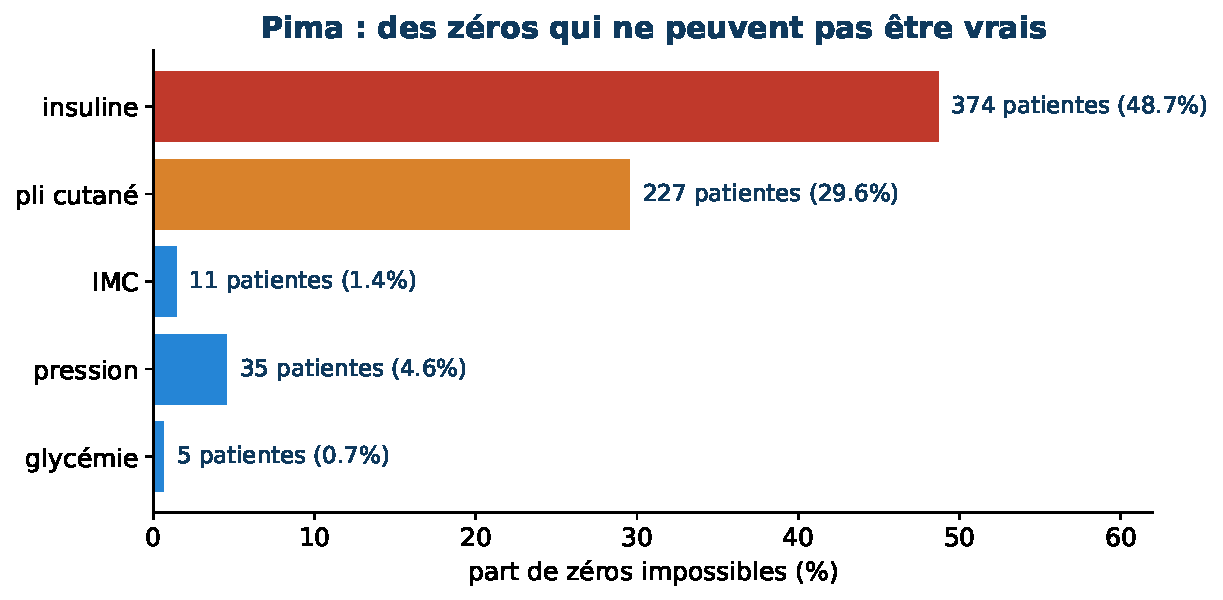
\includegraphics[width=0.62\linewidth]{f4_zeros}
\vspace{-2pt}

{\scriptsize Une glycémie de $0$ ou une pression artérielle de $0$ sont \emph{physiologiquement impossibles} : ce ne sont pas des mesures, ce sont des \textbf{absences de mesure} codées par un $0$. Près d'une patiente sur deux n'a pas de dosage d'insuline ($374/768$). Le fichier ne ment pas — il \emph{cache} ses trous.}
\end{frame}

\begin{frame}{La valeur manquante, formellement}
\begin{ucaddef}[Définition]
{\small Une \textbf{valeur manquante} est une case du tableau pour laquelle aucune mesure n'existe. Elle se note \texttt{NaN} (\emph{Not a Number}) — jamais $0$, qui est une valeur comme une autre. Le \textbf{taux de manquants} d'une colonne mesure l'ampleur du trou.}
\end{ucaddef}
\ucadformula{m_j \;=\; \frac{1}{n}\sum_{i=1}^{n} \mathbf{1}\big[x_{ij} \text{ manquant}\big]}
{\small La somme compte les cases vides de la colonne $j$ ; la division par $n$ en donne la proportion — exactement la mécanique du risque empirique de la Séance 3, appliquée aux trous plutôt qu'aux erreurs.}
\end{frame}

\begin{frame}{Exemple — les taux de manquants de Pima}
\begin{ucadex}[Après remplacement des zéros impossibles par NaN]
{\small \begin{center}\begin{tabular}{l|ccccc}
colonne & glycémie & pression & IMC & pli cutané & insuline\\\hline
manquants & $5$ & $35$ & $11$ & $227$ & $374$\\
$m_j$ & $0{,}007$ & $0{,}046$ & $0{,}014$ & $0{,}296$ & $\mathbf{0{,}487}$\\
\end{tabular}\end{center}
Pour l'insuline : $m = \dfrac{374}{768} = \mathbf{0{,}487}$ — près d'une case sur deux.}
\end{ucadex}
{\small Cinq colonnes touchées, à des degrés très différents : la réparation devra être \emph{automatique} et \emph{colonne par colonne}.}
\end{frame}

\begin{frame}{Exercice — calculer un taux de manquants}
\begin{ucadrec}[Énoncé]
{\small La colonne pression compte $35$ valeurs manquantes sur $768$ patientes. \textbf{(a)} Calculer $m_{\text{pression}}$. \textbf{(b)} Si l'on jetait toute ligne ayant \emph{au moins un} trou, il resterait $392$ patientes : quelle proportion du jeu perdrait-on ?}
\end{ucadrec}
\pause
\begin{ucadex}[Correction]
{\small \textbf{(a)} $m = \dfrac{35}{768} = \mathbf{0{,}046}$, soit $4{,}6\,\%$. \textbf{(b)} On perdrait $768 - 392 = 376$ patientes, soit $\dfrac{376}{768} = \mathbf{49\,\%}$ du jeu — la moitié des données sacrifiée pour des trous réparables.}
\end{ucadex}
\end{frame}

\begin{frame}{Piège — entraîner sur les zéros tels quels}
\begin{ucadpiege}[Erreur fréquente]
{\small Laisser les zéros impossibles dans les données. Le modèle apprend alors qu'il existe des patientes « à glycémie nulle » — une population fantôme — et place des coupures absurdes autour de $0$. Le score peut même sembler correct : le poison est \emph{silencieux}.}
\end{ucadpiege}
\begin{ucadpiege}[Erreur fréquente — bis]
{\small Jeter toutes les lignes incomplètes : ici, $49\,\%$ des patientes disparaîtraient. Pire, elles ne disparaissent pas \emph{au hasard} — les patientes sans dosage d'insuline sont souvent celles des structures les moins équipées : on biaiserait l'échantillon en croyant le nettoyer.}
\end{ucadpiege}
{\small La voie raisonnable : \textbf{garder les lignes, remplir les trous}. C'est l'imputation.}
\end{frame}

% #####################################################################
\section{Réparer : l'imputation par la médiane}

\begin{frame}{L'idée : remplir avec une valeur plausible}
\begin{ucaddef}[Le principe]
{\small \textbf{Imputer}, c'est remplacer chaque case vide d'une colonne par une valeur \emph{typique} de cette colonne. La question devient : quelle valeur typique ? La moyenne semble naturelle — mais elle a un défaut rédhibitoire sur les données médicales.}
\end{ucaddef}
\begin{ucadfront}[Analogie]
{\small Pour estimer le loyer « typique » d'un quartier, la moyenne se laisse entraîner par une seule villa de luxe ; le loyer \emph{médian} — celui du logement du milieu — reste fidèle au quartier. Les colonnes médicales ont leurs villas de luxe : les valeurs extrêmes.}
\end{ucadfront}
\end{frame}

\begin{frame}{La médiane, formellement}
\begin{ucaddef}[Définition]
{\small La \textbf{médiane} d'une colonne est la valeur du \emph{milieu} une fois les valeurs triées : la moitié des valeurs lui est inférieure, la moitié supérieure. Contrairement à la moyenne, elle est \textbf{robuste} : une valeur extrême ne la déplace presque pas.}
\end{ucaddef}
\begin{ucadex}[Exemple numérique — cinq insulines]
{\small Valeurs triées : $88$ ; $94$ ; $\mathbf{105}$ ; $130$ ; $480$. La médiane est la 3\textsuperscript{e} valeur : $\mathbf{105}$. La moyenne, elle, vaut $\dfrac{88+94+105+130+480}{5} = \mathbf{179{,}4}$ — tirée vers le haut par la seule valeur $480$, au point de dépasser $4$ patientes sur $5$.}
\end{ucadex}
\end{frame}

\begin{frame}{La robustesse, en image}
\centering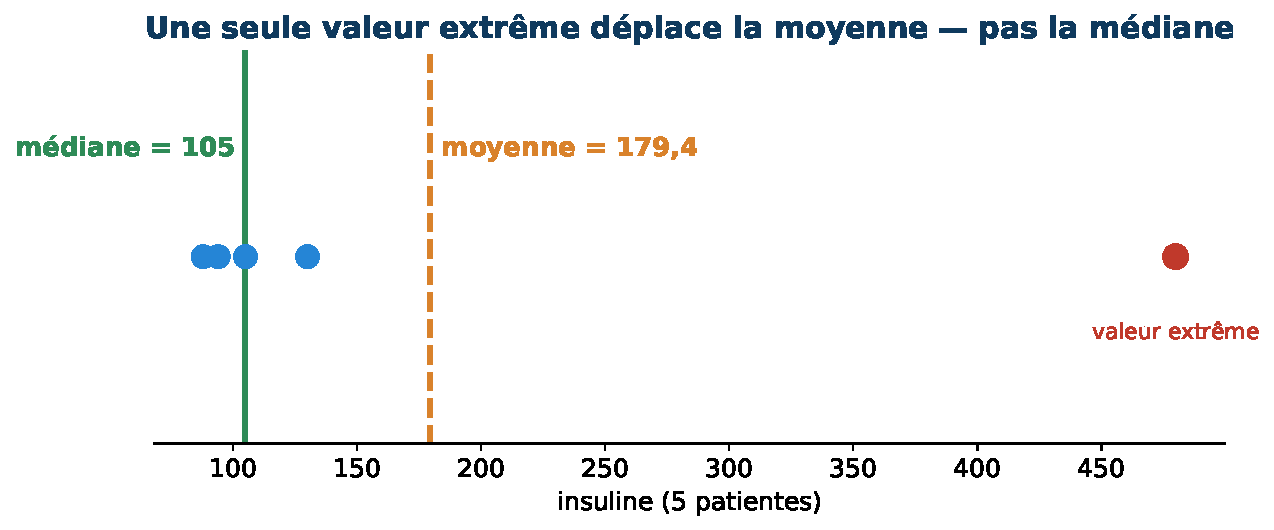
\includegraphics[width=0.72\linewidth]{f4_median}
\vspace{-2pt}

{\scriptsize Quatre patientes entre $88$ et $130$, une à $480$ : la moyenne ($179{,}4$) ne ressemble à \emph{aucune} patiente ; la médiane ($105$) reste au cœur du groupe. C'est elle qu'on injecte dans les trous.}
\end{frame}

\begin{frame}{L'imputation, formellement}
\begin{ucaddef}[Définition]
{\small L'\textbf{imputation par la médiane} remplace chaque valeur manquante de la colonne $j$ par la médiane $\text{med}_j$ de cette colonne — médiane calculée sur le \textbf{jeu d'entraînement uniquement}.}
\end{ucaddef}
\ucadformula{\tilde{x}_{ij} \;=\; \begin{cases} x_{ij} & \text{si } x_{ij} \text{ est observée}\\[2pt] \text{med}_j & \text{si } x_{ij} \text{ est manquante} \end{cases}}
{\small Point décisif : $\text{med}_j$ est un \textbf{paramètre appris} des données, au même titre que les coupures de l'arbre. Et comme tout paramètre appris, il s'apprend sur le train — \emph{jamais} sur le test. La raison précise arrive à la section « fuite de données ».}
\end{frame}

\begin{frame}{Exemple — l'imputation en chiffres sur Pima}
\begin{ucadex}[Médianes apprises sur le train]
{\small Sur les $614$ patientes d'entraînement : $\text{med}_{\text{insuline}} = \mathbf{125{,}5}$, $\text{med}_{\text{glycémie}} = 118{,}0$, $\text{med}_{\text{IMC}} = 32{,}0$.\\[3pt]
La patiente n°$525$ (du test) a une insuline manquante : $\tilde{x}_{525,\,\text{insuline}} = \text{med}_{\text{insuline}} = \mathbf{125{,}5}$. Ses valeurs observées (glycémie $87$, âge $21$) restent intactes.}
\end{ucadex}
{\small À comparer : la \emph{moyenne} de l'insuline sur le train vaut $139{,}4$ — gonflée par les valeurs extrêmes, elle aurait rempli les trous avec une valeur peu typique.}
\end{frame}

\begin{frame}{Exercice — imputer à la main}
\begin{ucadrec}[Énoncé]
{\small Une mini-colonne IMC contient : $24{,}1$ ; \texttt{NaN} ; $31{,}5$ ; $28{,}0$ ; \texttt{NaN} ; $35{,}2$. \textbf{(a)} Calculer la médiane des valeurs observées. \textbf{(b)} Donner la colonne imputée.}
\end{ucadrec}
\pause
\begin{ucadex}[Correction]
{\small \textbf{(a)} Valeurs observées triées : $24{,}1$ ; $28{,}0$ ; $31{,}5$ ; $35{,}2$ — nombre pair, la médiane est la moyenne des deux du milieu : $\dfrac{28{,}0 + 31{,}5}{2} = \mathbf{29{,}75}$. \textbf{(b)} Colonne imputée : $24{,}1$ ; $\mathbf{29{,}75}$ ; $31{,}5$ ; $28{,}0$ ; $\mathbf{29{,}75}$ ; $35{,}2$ — les valeurs observées ne bougent pas.}
\end{ucadex}
\end{frame}

\begin{frame}[fragile]{En pratique : SimpleImputer}
\begin{lstlisting}
import numpy as np
from sklearn.impute import SimpleImputer

X[colonnes_impossibles] = X[colonnes_impossibles].replace(0, np.nan)
imputeur = SimpleImputer(strategy="median")
imputeur.fit(X_train)                  # apprend les medianes (train !)
X_train_p = imputeur.transform(X_train)
X_test_p  = imputeur.transform(X_test) # applique les MEMES medianes
\end{lstlisting}
{\small Le motif \texttt{fit} / \texttt{transform} est le cœur de toute la séance : \texttt{fit} \emph{apprend} les paramètres (ici, une médiane par colonne), \texttt{transform} les \emph{applique}. Le test ne voit jamais \texttt{fit} — il ne fait que subir \texttt{transform}.}
\end{frame}

% #####################################################################
\section{Encoder les catégories}

\begin{frame}{Le problème : les modèles mangent des nombres}
\begin{ucaddef}[Le constat]
{\small Distances, seuils, moyennes : tout ce que manipule un modèle est \textbf{numérique}. Or les données réelles portent des \textbf{catégories} — une région ($\{$Dakar, Thiès, Kaolack, Ziguinchor, Saint-Louis$\}$), un sexe, un type d'admission. Il faut les traduire en nombres \emph{sans inventer d'information}.}
\end{ucaddef}
\begin{ucadpiege}[Erreur fréquente]
{\small Coder Dakar $=1$, Thiès $=2$, \dots, Saint-Louis $=5$. Ces entiers fabriquent un \textbf{ordre fictif} (Saint-Louis $>$ Dakar ?) et de fausses distances (Kaolack serait « deux fois plus loin » de Dakar que Thiès). Le modèle prendra cette géométrie inventée au sérieux.}
\end{ucadpiege}
\end{frame}

\begin{frame}{L'encodage one-hot, formellement}
\begin{ucaddef}[Définition]
{\small L'encodage \textbf{one-hot} remplace une colonne à $K$ modalités par $K$ colonnes binaires : la colonne de la modalité observée vaut $1$, toutes les autres $0$. Aucun ordre, aucune distance fictive — chaque modalité est à égale distance de toutes les autres.}
\end{ucaddef}
\begin{ucadex}[Exemple — la région en cinq colonnes]
{\small \begin{center}\begin{tabular}{l|ccccc}
région & Dakar & Thiès & Kaolack & Ziguinchor & Saint-Louis\\\hline
« Thiès » & $0$ & $\mathbf{1}$ & $0$ & $0$ & $0$\\
« Saint-Louis » & $0$ & $0$ & $0$ & $0$ & $\mathbf{1}$\\
\end{tabular}\end{center}
Une seule colonne « chaude » (\emph{hot}) par ligne — d'où le nom.}
\end{ucadex}
\end{frame}

\begin{frame}{Exercice — encoder à la main}
\begin{ucadrec}[Énoncé]
{\small Une colonne « type d'admission » a $4$ modalités : urgences, consultation, transfert, programmée. \textbf{(a)} Combien de colonnes produit le one-hot ? \textbf{(b)} Encoder « transfert ». \textbf{(c)} Pourquoi ne pas coder simplement $1, 2, 3, 4$ ?}
\end{ucadrec}
\pause
\begin{ucadex}[Correction]
{\small \textbf{(a)} $4$ colonnes binaires. \textbf{(b)} $(0,\ 0,\ \mathbf{1},\ 0)$. \textbf{(c)} Les entiers imposeraient un ordre et des écarts inventés — « programmée » ($4$) serait \emph{trois fois plus loin} des urgences ($1$) que « consultation » ($2$), une géométrie qui ne correspond à rien de médical et que les distances de la section suivante prendraient au pied de la lettre.}
\end{ucadex}
\end{frame}

% #####################################################################
\section{Mettre à l'échelle : la standardisation}

\begin{frame}{Le problème des échelles}
\begin{ucaddef}[Le constat sur Pima]
{\small L'âge court de $21$ à $81$ ; l'insuline de $14$ à $846$. Les deux colonnes parlent des unités incomparables — et tout calcul qui les \emph{mélange} (une distance, une somme pondérée) sera dominé par la colonne aux grands nombres, indépendamment de son intérêt médical.}
\end{ucaddef}
\begin{ucadfront}[Analogie]
{\small Comparer des prix en francs CFA et en euros sans convertir : celui en francs « pèse » des centaines de fois plus dans toute addition — non parce qu'il est plus cher, mais parce que son unité est plus petite. La standardisation est cette conversion : tout le monde dans la même monnaie.}
\end{ucadfront}
\end{frame}

\begin{frame}{Le z-score, formellement}
\begin{ucaddef}[Définition]
{\small \textbf{Standardiser} une colonne, c'est la recentrer sur $0$ et la réduire à un écart-type de $1$ : chaque valeur devient son \textbf{z-score} — sa distance à la moyenne, \emph{comptée en écarts-types}.}
\end{ucaddef}
\ucadformula{z \;=\; \frac{x - \mu}{\sigma}}
{\small $\mu$ et $\sigma$ sont la moyenne et l'écart-type de la colonne, \textbf{appris sur le train}. Lecture : $z = 0$, valeur parfaitement moyenne ; $z = +2$, deux écarts-types au-dessus — grand, quelle que soit l'unité d'origine. Toutes les colonnes parlent désormais la même langue.}
\end{frame}

\begin{frame}{Exemple — un z-score en chiffres}
\begin{ucadex}[La glycémie sur le train de Pima]
{\small Sur les $614$ patientes d'entraînement : $\mu_{\text{glycémie}} = 121{,}6$ et $\sigma_{\text{glycémie}} = 30{,}0$.\\[3pt]
Une patiente à glycémie $180$ : $z = \dfrac{180 - 121{,}6}{30{,}0} = \dfrac{58{,}4}{30{,}0} = \mathbf{1{,}95}$ — presque deux écarts-types au-dessus de la moyenne : nettement élevée.}
\end{ucadex}
{\small Même opération pour chaque colonne avec \emph{ses} $\mu$ et $\sigma$ : l'insuline ($\mu = 139{,}4$, $\sigma = 84{,}4$) et l'âge ($\mu = 33{,}6$, $\sigma = 11{,}9$) deviennent comparables terme à terme.}
\end{frame}

\begin{frame}{Exercice — standardiser à la main}
\begin{ucadrec}[Énoncé]
{\small Sur le train, l'âge a pour moyenne $\mu = 33{,}6$ et pour écart-type $\sigma = 11{,}9$. Calculer le z-score d'une patiente de $57$ ans, et interpréter.}
\end{ucadrec}
\pause
\begin{ucadex}[Correction]
{\small $z = \dfrac{57 - 33{,}6}{11{,}9} = \dfrac{23{,}4}{11{,}9} = \mathbf{1{,}97}$ — environ deux écarts-types au-dessus de la moyenne : cette patiente est nettement plus âgée que la population du registre, exactement comme la glycémie $180$ l'était pour sa colonne. Les deux $z$ se comparent directement : c'est tout l'intérêt.}
\end{ucadex}
\end{frame}

\begin{frame}{Avant / après, en image}
\centering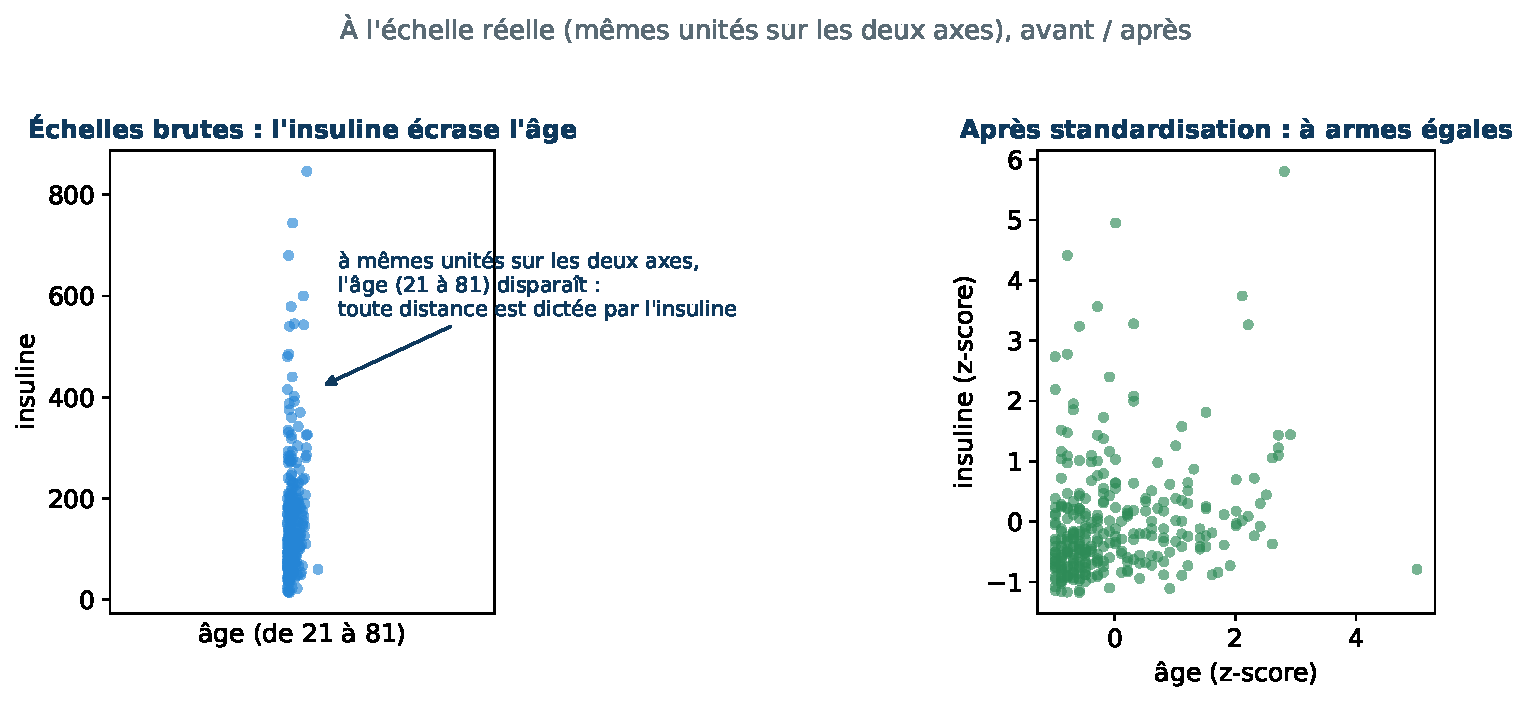
\includegraphics[width=0.82\linewidth]{f4_scale}
\vspace{-2pt}

{\scriptsize À gauche, âge et insuline tracés \emph{dans les mêmes unités} : l'âge disparaît, toute distance entre patientes est dictée par l'insuline. À droite, après standardisation : les deux variables pèsent selon leurs écarts réels. L'arbre de la Séance 3, qui coupe colonne par colonne, n'y était pas sensible — le modèle qui arrive l'est \emph{viscéralement}.}
\end{frame}

% #####################################################################
\section{Un second modèle : les k plus proches voisins}

\begin{frame}{L'idée : on prédit comme ses semblables}
\begin{ucadfront}[Analogie]
{\small Pour estimer un loyer, un courtier ne résout pas d'équation : il regarde les maisons \emph{voisines et comparables}, et annonce un loyer semblable. Les $k$ plus proches voisins automatisent ce réflexe : « les patientes au profil proche ont connu telle issue ».}
\end{ucadfront}
\centering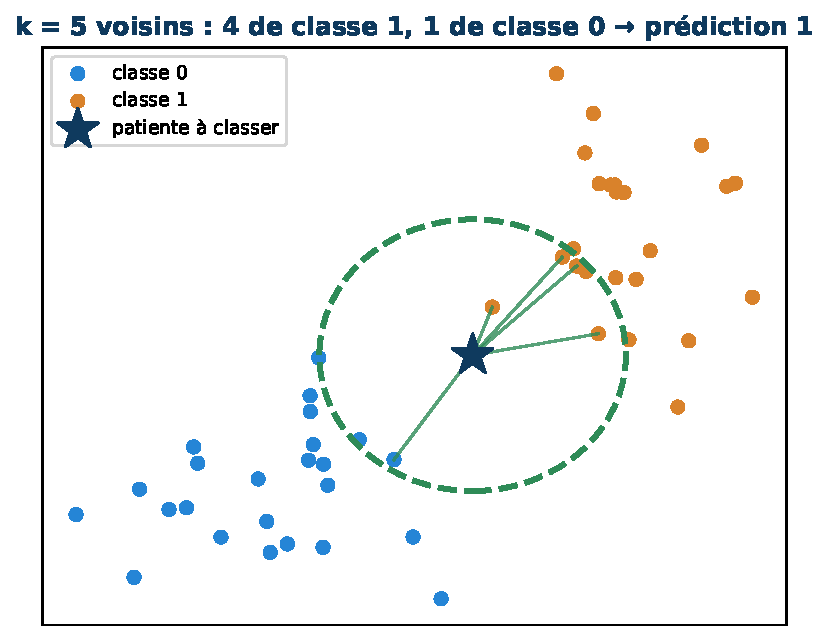
\includegraphics[width=0.30\linewidth]{f4_knn}
\vspace{-2pt}

{\scriptsize Classer la patiente $\star$ : trouver ses $k=5$ voisines, prendre la classe \textbf{majoritaire} — ici $4$ contre $1$, prédiction $1$.}
\end{frame}

\begin{frame}{La distance euclidienne, formellement}
\begin{ucaddef}[Mesurer la proximité]
{\small « Proche » exige une \textbf{distance}. La distance euclidienne entre deux patientes est la longueur du segment qui les relie dans l'espace des caractéristiques — le théorème de Pythagore, en dimension $d$.}
\end{ucaddef}
\ucadformula{d(x, x') \;=\; \sqrt{\sum_{j=1}^{d} \big(x_j - x'_j\big)^2}}
\begin{ucadex}[Exemple numérique]
{\small En dimension $2$ : $d\big((3,4),\,(0,0)\big) = \sqrt{3^2 + 4^2} = \sqrt{9+16} = \sqrt{25} = \mathbf{5}$. Chaque caractéristique contribue par son écart \emph{au carré} — un grand écart sur une seule colonne suffit à dominer toute la somme. Retenir ce détail : il explique tout ce qui suit.}
\end{ucadex}
\end{frame}

\begin{frame}{Le modèle kNN, formellement}
\begin{ucaddef}[Définition]
{\small Le modèle des \textbf{$k$ plus proches voisins} prédit, pour une entrée $x$, la classe \textbf{majoritaire} parmi les $k$ exemples d'entraînement les plus proches de $x$.}
\end{ucaddef}
\ucadformula{f(x) \;=\; \text{majorité}\big\{\, y_i \;:\; x_i \in V_k(x) \,\big\}}
{\small $V_k(x)$ est l'ensemble des $k$ voisins les plus proches de $x$ dans le jeu d'entraînement. Particularité frappante : il n'y a \emph{rien à entraîner} — \texttt{fit} se contente de \textbf{mémoriser} les exemples ; tout le travail (calculer les distances, voter) a lieu au moment de \texttt{predict}. C'est l'exact opposé de l'arbre, qui travaille à l'entraînement et prédit en un éclair.}
\end{frame}

\begin{frame}{Exemple — classer à la main avec $k=3$}
\begin{ucadex}[Cinq voisines connues, une patiente à classer en x égal (4 ; 4)]
{\small \begin{center}\begin{tabular}{c|cc|c|c}
voisine & coord. & classe & distance à $(4,4)$ & rang\\\hline
$A$ & $(5,5)$ & $1$ & $\sqrt{1+1} = 1{,}41$ & 1\textsuperscript{er}\\
$B$ & $(2,4)$ & $0$ & $\sqrt{4+0} = 2{,}00$ & 2\textsuperscript{e}\\
$C$ & $(6,3)$ & $1$ & $\sqrt{4+1} = 2{,}24$ & 3\textsuperscript{e}\\
$D$ & $(1,1)$ & $0$ & $\sqrt{9+9} = 4{,}24$ & —\\
$E$ & $(7,7)$ & $1$ & $\sqrt{9+9} = 4{,}24$ & —\\
\end{tabular}\end{center}
$V_3 = \{A, B, C\}$, classes $\{1, 0, 1\}$ : majorité $\mathbf{1}$ — $f\big((4,4)\big) = 1$.}
\end{ucadex}
\end{frame}

\begin{frame}{Exercice — refaire le vote avec $k=5$}
\begin{ucadrec}[Énoncé]
{\small Mêmes cinq voisines, même patiente $(4,4)$. Donner la prédiction pour $k = 5$, puis expliquer pourquoi on choisit presque toujours $k$ \emph{impair} en classification binaire.}
\end{ucadrec}
\pause
\begin{ucadex}[Correction]
{\small $V_5$ = toutes les voisines, classes $\{1, 0, 1, 0, 1\}$ : trois voix contre deux, prédiction $\mathbf{1}$. Un $k$ pair autoriserait des votes à égalité ($2$–$2$), qu'il faudrait trancher arbitrairement ; un $k$ impair garantit toujours une majorité nette.}
\end{ucadex}
\end{frame}

\begin{frame}{Pourquoi l'échelle est une condition de validité}
\begin{ucadex}[Trois patientes en deux mesures — âge et insuline]
{\small $A = (25,\ 100)$, \quad $B = (26,\ 400)$, \quad $C = (60,\ 105)$. Qui est la plus proche de $A$ ?\\[3pt]
\textbf{En brut} : $d(A,B) = \sqrt{1^2 + 300^2} = \mathbf{300{,}0}$ ; \; $d(A,C) = \sqrt{35^2 + 5^2} = \mathbf{35{,}4}$ — la sexagénaire $C$ paraît $8$ fois plus proche de la jeune $A$ que $B$, son quasi-jumeau d'âge : \textbf{l'insuline a tout écrasé}.\\[3pt]
\textbf{Standardisé} (avec les $\mu, \sigma$ du train, après imputation) : $d(A,B) = \mathbf{3{,}55}$ ; \; $d(A,C) = \mathbf{2{,}95}$ — l'ordre s'inverse, $B$ redevient la plus proche, chaque variable pesant selon ses écarts réels.}
\end{ucadex}
{\small Sur Pima en entier, le verdict chiffré : kNN ($k=5$) \textbf{sans} standardisation $= 0{,}714$ ; \textbf{avec} $= \mathbf{0{,}727}$. Pour un modèle à distances, la mise à l'échelle n'est pas un raffinement — c'est une \textbf{condition de validité} du calcul lui-même.}
\end{frame}

\begin{frame}{Le réglage $k$ : la complexité, encore elle}
\centering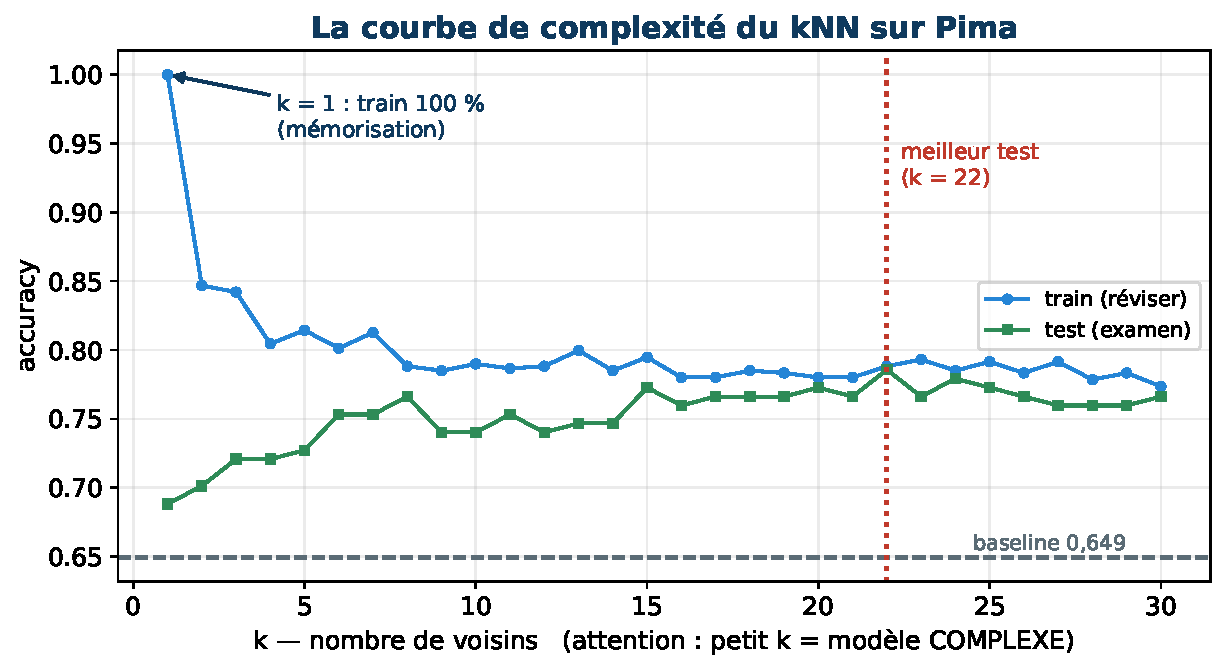
\includegraphics[width=0.62\linewidth]{f4_kcurve}
\vspace{-2pt}

{\scriptsize Attention au sens de lecture : \textbf{petit $k$ = modèle complexe}. À $k=1$, chaque patiente du train est sa propre voisine — train $100\,\%$, test $0{,}688$ : pure mémorisation, le tailleur qui recoud à chaque essayage (\textbf{variance}). À $k$ très grand, le vote noie tout détail local — le patron unique (\textbf{biais}). Le meilleur test : $k = 22$, accuracy $\mathbf{0{,}786}$.}
\end{frame}

\begin{frame}{Exercice — diagnostiquer par la paire de scores}
\begin{ucadrec}[Énoncé]
{\small Trois réglages du kNN sur Pima : \textbf{A} $k=1$ : $(1{,}000;\ 0{,}688)$ ; \textbf{B} $k=22$ : $(0{,}79;\ 0{,}786)$ ; \textbf{C} $k=300$ : scores faibles et proches tous les deux. Diagnostiquer chacun avec le vocabulaire de la Séance 3.}
\end{ucadrec}
\pause
\begin{ucadex}[Correction]
{\small \textbf{A} : écart majeur train/test — \textbf{sur-apprentissage} (variance) ; mémoriser ses voisines n'est pas généraliser. \textbf{B} : scores corrects et proches — le bon compromis. \textbf{C} : avec $300$ voisines sur $614$, le vote tend vers la classe majoritaire globale — \textbf{sous-apprentissage} (biais), le modèle redevient presque la baseline. La grille de lecture de la Séance 3 s'applique mot pour mot : seul le bouton de complexité a changé de nom.}
\end{ucadex}
\end{frame}

% #####################################################################
\section{La fuite de données}

\begin{frame}{L'idée : un examen dont les questions ont fuité}
\begin{ucadfront}[Analogie]
{\small Un étudiant obtient $20/20$ — puis on découvre que le sujet de l'examen avait circulé la veille. Sa note ne mesure plus sa compréhension : elle mesure la fuite. En ML, le « sujet » est le jeu de test : toute information qui s'en échappe vers l'apprentissage fabrique un score menteur.}
\end{ucadfront}
\begin{ucaddef}[Définition]
{\small Il y a \textbf{fuite de données} (\emph{data leakage}) lorsque l'apprentissage utilise une information qui ne sera \textbf{pas disponible au moment de la prédiction} — ou qui provient du jeu de test. Le score mesuré est alors trop beau, et le modèle déployé déçoit.}
\end{ucaddef}
{\small Deux familles : la \textbf{variable fuyarde} (une colonne qui contient la réponse) et le \textbf{prétraitement fuyard} (des paramètres appris sur le test). Démonstration de chacune.}
\end{frame}

\begin{frame}{Fuite n°1 — la variable fuyarde}
\begin{ucadex}[La démonstration sur Pima]
{\small Ajoutons une colonne « \texttt{traitement} » ($1$ si un traitement antidiabétique a été prescrit). L'arbre, réentraîné : accuracy $= \mathbf{1{,}000}$. Parfait ? Non — le traitement vient \emph{après} le diagnostic : la colonne \textbf{contient la réponse}, et à l'admission, au moment de prédire, elle n'existera pas.}
\end{ucadex}
\centering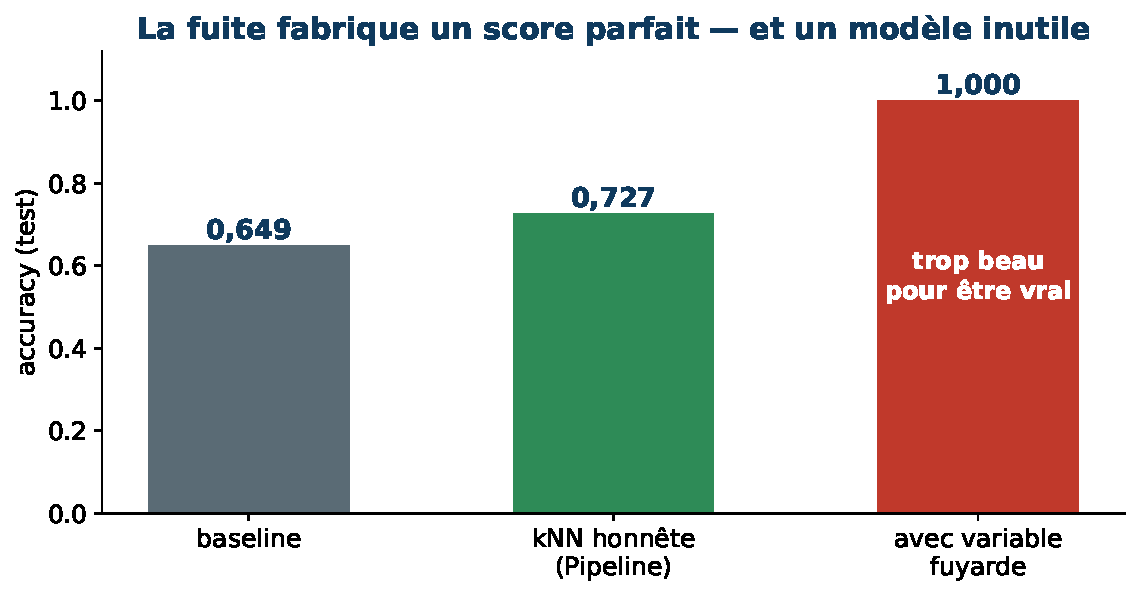
\includegraphics[width=0.42\linewidth]{f4_leak}
\vspace{-2pt}

{\scriptsize Le test à appliquer à \emph{chaque} colonne : « cette information existera-t-elle \textbf{au moment de prédire} ? » Si non, elle sort — quel que soit le score qu'elle promet.}
\end{frame}

\begin{frame}{Fuite n°2 — le prétraitement fuyard}
\begin{ucaddef}[Le mécanisme]
{\small Médianes, $\mu$, $\sigma$ : tous les paramètres de préparation sont \emph{appris}. Les apprendre sur le jeu \textbf{complet} — test inclus — c'est laisser le test influencer l'apprentissage : le modèle a « vu » la moyenne de l'examen avant de le passer.}
\end{ucaddef}
\begin{ucadex}[Sur Pima — un poison discret]
{\small Protocole fuyard (standardisation apprise sur les $768$ patientes, split ensuite) : $0{,}727$. Protocole honnête : $0{,}727$ aussi — ici, l'écart est \emph{invisible}. C'est précisément ce qui rend cette fuite dangereuse : elle ne se voit pas au score, le protocole ment \emph{par construction}, et sur d'autres jeux (séries temporelles, petits échantillons) l'écart devient majeur. La règle ne se négocie pas au cas par cas : \textbf{tout \texttt{fit} se fait sur le train}.}
\end{ucadex}
\end{frame}

\begin{frame}{Exercice — repérer la fuite}
\begin{ucadrec}[Énoncé]
{\small Pour chaque protocole, dire s'il y a fuite et laquelle : \textbf{(a)} prédire une réadmission avec la colonne « durée totale du séjour » ; \textbf{(b)} standardiser tout le jeu, puis faire le split train/test ; \textbf{(c)} imputer le train avec les médianes du train, puis le test avec \emph{ces mêmes} médianes.}
\end{ucadrec}
\pause
\begin{ucadex}[Correction]
{\small \textbf{(a)} Variable fuyarde : la durée n'est connue qu'\emph{à la sortie} — au moment de prédire la réadmission, elle n'existe pas encore sous sa forme finale. \textbf{(b)} Prétraitement fuyard : $\mu$ et $\sigma$ ont vu le test. \textbf{(c)} \textbf{Aucune fuite} — c'est exactement le bon protocole : paramètres appris sur le train, appliqués tels quels au test. Appliquer n'est pas apprendre.}
\end{ucadex}
\end{frame}

% #####################################################################
\section{Le Pipeline : souder la chaîne}

\begin{frame}{L'idée : une seule chaîne, soudée}
\centering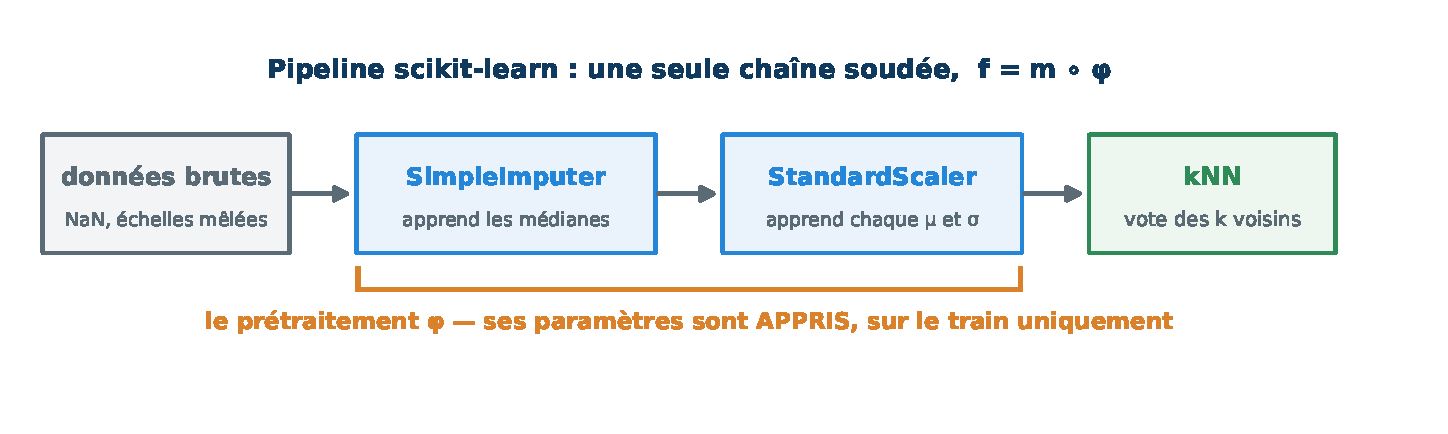
\includegraphics[width=0.92\linewidth]{f4_pipeline}
\vspace{-2pt}

{\scriptsize Imputer, standardiser, prédire : trois maillons, chacun avec ses paramètres appris. Les enchaîner à la main multiplie les occasions de fuite (un \texttt{fit} de trop, un ordre inversé). Le \textbf{Pipeline} soude la chaîne : un seul \texttt{fit} (sur le train), un seul \texttt{predict} — la fuite de prétraitement devient \emph{impossible par construction}.}
\end{frame}

\begin{frame}{Le Pipeline, formellement}
\begin{ucaddef}[Définition]
{\small Le modèle complet est la \textbf{composée} d'un prétraitement $\varphi$ et d'un prédicteur $m$ : d'abord transformer, ensuite prédire. Le prétraitement porte ses propres paramètres appris $\theta_\varphi$ — les médianes, les $\mu$ et les $\sigma$.}
\end{ucaddef}
\ucadformula{f(x) \;=\; m\big(\varphi(x)\big) \qquad \text{avec } \theta_\varphi \text{ appris sur le train uniquement}}
{\small Lire de droite à gauche, comme toute composée : $x$ entre, $\varphi$ le répare et le met à l'échelle, $m$ prédit. Le \texttt{fit} du Pipeline apprend \emph{tout} d'un coup — $\theta_\varphi$ puis les paramètres de $m$ — sur les mêmes données d'entraînement ; le test ne traverse la chaîne qu'en \texttt{transform} et \texttt{predict}.}
\end{frame}

\begin{frame}{Exemple — $\varphi(x)$ pas à pas sur une patiente}
\begin{ucadex}[La patiente n°525 du test traverse la chaîne]
{\small \begin{center}\small\begin{tabular}{l|ccc}
étape & glycémie & insuline & âge\\\hline
brut & $87$ & \texttt{NaN} & $21$\\
après imputation & $87$ & $\mathbf{125{,}5}$ & $21$\\
après z-score & $\dfrac{87-121{,}6}{30{,}0} = \mathbf{-1{,}16}$ & $\dfrac{125{,}5-139{,}4}{84{,}4} = \mathbf{-0{,}16}$ & $\dfrac{21-33{,}6}{11{,}9} = \mathbf{-1{,}06}$\\
\end{tabular}\end{center}
Chaque nombre utilisé ($125{,}5$ ; $121{,}6$ ; $30{,}0$ ; \dots) vient du \textbf{train} : la patiente, elle, est du test — elle subit la chaîne, elle ne l'a jamais nourrie. Puis $m$ (le kNN) vote sur ce vecteur réparé : $f(x) = m\big(\varphi(x)\big)$.}
\end{ucadex}
\end{frame}

\begin{frame}[fragile]{En pratique : Pipeline scikit-learn}
\begin{lstlisting}
from sklearn.pipeline import Pipeline
from sklearn.impute import SimpleImputer
from sklearn.preprocessing import StandardScaler
from sklearn.neighbors import KNeighborsClassifier

modele = Pipeline([
    ("imputation", SimpleImputer(strategy="median")),
    ("echelle",    StandardScaler()),
    ("knn",        KNeighborsClassifier(n_neighbors=22)),
])
modele.fit(X_train, y_train)     # UN fit : medianes, mu/sigma, voisins
modele.score(X_test, y_test)     # 0.786
\end{lstlisting}
{\small Le triptyque \texttt{fit} / \texttt{predict} / \texttt{score} de la Séance 3, inchangé — le Pipeline \emph{est} un modèle comme les autres. Toute la discipline anti-fuite tient dans ces deux lignes finales.}
\end{frame}

\begin{frame}{Le bilan chiffré de la séance}
\begin{ucadex}[Tous les scores sur le même test — 154 patientes]
{\small \begin{center}\begin{tabular}{l c}
modèle & accuracy (test)\\\hline
baseline (classe majoritaire) & $0{,}649$\\
arbre profondeur $4$ + imputation & $0{,}662$\\
kNN $k=5$ \emph{sans} standardisation & $0{,}714$\\
kNN $k=5$, Pipeline complet & $0{,}727$\\
kNN $k=22$, Pipeline complet & $\mathbf{0{,}786}$\\
\emph{n'importe quoi} + variable fuyarde & \emph{1{,}000 — mensonge}\\
\end{tabular}\end{center}}
\end{ucadex}
{\small \textbf{Deux leçons.} Le kNN bien préparé bat nettement l'arbre — \textbf{aucun modèle n'est roi partout}. Et le saut de $0{,}662$ à $0{,}786$ ne tient pas à un coup de génie : la standardisation rend la distance du kNN \emph{valide} ($0{,}714 \to 0{,}727$), le choix de modèle et le réglage de $k$ font le
reste — la \textbf{méthodologie}, pas la chance.}
\end{frame}


\begin{frame}{Exercice — remettre la chaîne dans l'ordre}
\begin{ucadrec}[Énoncé]
{\small Remettre dans l'ordre les cinq étapes d'une étude propre : \textbf{(1)} \texttt{score} sur le test ; \textbf{(2)} \texttt{train\_test\_split} ; \textbf{(3)} remplacer les zéros impossibles par \texttt{NaN} ; \textbf{(4)} \texttt{fit} du Pipeline sur le train ; \textbf{(5)} construire le Pipeline (imputation $\to$ échelle $\to$ modèle). Où une inversion $2 \leftrightarrow 4$ créerait-elle une fuite ?}
\end{ucadrec}
\pause
\begin{ucadex}[Correction]
{\small Ordre : $\mathbf{3 \to 2 \to 5 \to 4 \to 1}$. (Le remplacement $0 \to$ \texttt{NaN} n'apprend rien — il peut précéder le split.) Inverser $2$ et $4$, c'est \texttt{fit} avant le découpage : médianes, $\mu$ et $\sigma$ appris sur les $768$ patientes, test compris — la fuite n°2 exactement. Le split vient toujours \emph{avant} tout \texttt{fit}.}
\end{ucadex}
\end{frame}

% #####################################################################
\section{Synthèse}

\begin{frame}{Le protocole complet, version 2}
\begin{ucadret}[De bout en bout — mis à jour]
{\small \textbf{1.} Formuler : $(X, y)$. \;\textbf{2.} \textbf{Auditer} : zéros impossibles $\to$ \texttt{NaN}, taux de manquants, échelles, colonnes fuyardes. \;\textbf{3.} Découper : \texttt{train\_test\_split}. \;\textbf{4.} Construire le \textbf{Pipeline} : imputation $\to$ encodage $\to$ standardisation $\to$ modèle. \;\textbf{5.} \texttt{fit} sur le train — un seul, celui du Pipeline. \;\textbf{6.} \texttt{score} sur le test, contre la baseline. \;\textbf{7.} Diagnostiquer : paire (train, test), réglage de la complexité ($k$, profondeur).}
\end{ucadret}
{\small L'étape $2$ est la nouveauté profonde de la séance : avant cette séance, on modélisait ; désormais, on \textbf{audite avant de modéliser}.}
\end{frame}

\begin{frame}{À retenir — Séance 4}
\begin{ucadret}[L'essentiel]
\begin{itemize}\small
  \item Les données réelles cachent leurs trous (zéros impossibles) ; on les expose (\texttt{NaN}, taux $m_j$) puis on les répare par la \textbf{médiane} — robuste aux valeurs extrêmes — apprise sur le train.
  \item Les catégories s'encodent en \textbf{one-hot} ; les échelles s'alignent par le \textbf{z-score} $z = (x-\mu)/\sigma$.
  \item Le \textbf{kNN} prédit par vote des $k$ voisins : sans mise à l'échelle, sa distance est dominée par les grandes colonnes — l'échelle est une \emph{condition de validité}. Petit $k$ = variance, grand $k$ = biais.
  \item La \textbf{fuite de données} fabrique des scores menteurs : variable fuyarde (la réponse déguisée) ou prétraitement fuyard (\texttt{fit} hors du train).
  \item Le \textbf{Pipeline} soude $f = m \circ \varphi$ : un seul \texttt{fit}, sur le train — la fuite de prétraitement devient impossible par construction.
\end{itemize}
\end{ucadret}
\end{frame}

\begin{frame}{Pièges fréquents}
\begin{itemize}\small
  \item Prendre les zéros impossibles pour des mesures — ou jeter la moitié du jeu pour s'en débarrasser.
  \item Imputer par la moyenne sur des colonnes à valeurs extrêmes ($179{,}4$ contre $105$ : la moyenne ne ressemble à personne).
  \item Encoder des catégories par des entiers ordonnés : une géométrie inventée que les distances prennent au sérieux.
  \item Nourrir un kNN de colonnes non standardisées : la distance n'écoute plus que les grands nombres.
  \item Croire un score parfait : $1{,}000$ n'est pas une victoire, c'est une \textbf{alarme} — chercher la colonne fuyarde.
  \item Faire un \texttt{fit} (imputeur, scaler) avant le split, ou un \texttt{fit\_transform} sur le test : tout \texttt{fit} vit sur le train.
\end{itemize}
\end{frame}

\begin{frame}{Prochaine séance}
\begin{ucadfront}[Séance 5 — Prédire un nombre : la régression]
{\small Jusqu'ici, la cible était une classe. La Séance 5 prédit une \textbf{quantité} — une durée de séjour en jours — avec la régression linéaire : ses coefficients lisibles, ses métriques propres (MAE, RMSE, R²), et le même Pipeline, devenu indispensable : la régression linéaire \emph{refuse} les \texttt{NaN}.}
\end{ucadfront}
\end{frame}

\begin{frame}{Références}
\begin{itemize}\small
  \item A. Géron, \emph{Hands-On Machine Learning with Scikit-Learn, Keras \& TensorFlow}, 3\textsuperscript{e} éd., O'Reilly, 2022.
  \item A. C. Müller, S. Guido, \emph{Introduction to Machine Learning with Python}, O'Reilly, 2016.
  \item G. James, D. Witten, T. Hastie, R. Tibshirani, \emph{An Introduction to Statistical Learning}, 2\textsuperscript{e} éd., Springer, 2021.
  \item J. W. Smith \emph{et al.}, « Using the ADAP learning algorithm to forecast the onset of diabetes mellitus », 1988 — le jeu Pima.
  \item Cours : Stanford CS229 ; Cornell CS4780.
\end{itemize}
\end{frame}

\end{document}
